% Created by tikzDevice version 0.12.6 on 2025-04-07 16:44:32
% !TEX encoding = UTF-8 Unicode
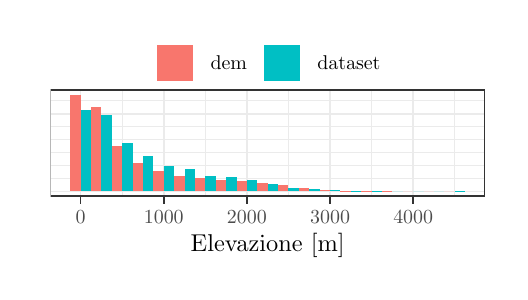
\begin{tikzpicture}[x=1pt,y=1pt]
\definecolor{fillColor}{RGB}{255,255,255}
\path[use as bounding box,fill=fillColor] (0,0) rectangle (170.72, 88.20);
\begin{scope}
\path[clip] (  0.00,  0.00) rectangle (170.72, 88.20);
\definecolor{drawColor}{RGB}{255,255,255}

\path[draw=drawColor,line width= 0.6pt,line join=round,line cap=round,fill=fillColor] (  0.00,  0.00) rectangle (170.72, 88.20);
\end{scope}
\begin{scope}
\path[clip] (  8.25, 27.29) rectangle (165.22, 65.79);
\definecolor{fillColor}{RGB}{255,255,255}

\path[fill=fillColor] (  8.25, 27.29) rectangle (165.22, 65.79);
\definecolor{drawColor}{gray}{0.92}

\path[draw=drawColor,line width= 0.3pt,line join=round] (  8.25, 33.71) --
	(165.22, 33.71);

\path[draw=drawColor,line width= 0.3pt,line join=round] (  8.25, 43.07) --
	(165.22, 43.07);

\path[draw=drawColor,line width= 0.3pt,line join=round] (  8.25, 52.42) --
	(165.22, 52.42);

\path[draw=drawColor,line width= 0.3pt,line join=round] (  8.25, 61.77) --
	(165.22, 61.77);

\path[draw=drawColor,line width= 0.3pt,line join=round] ( 34.16, 27.29) --
	( 34.16, 65.79);

\path[draw=drawColor,line width= 0.3pt,line join=round] ( 64.20, 27.29) --
	( 64.20, 65.79);

\path[draw=drawColor,line width= 0.3pt,line join=round] ( 94.24, 27.29) --
	( 94.24, 65.79);

\path[draw=drawColor,line width= 0.3pt,line join=round] (124.29, 27.29) --
	(124.29, 65.79);

\path[draw=drawColor,line width= 0.3pt,line join=round] (154.33, 27.29) --
	(154.33, 65.79);

\path[draw=drawColor,line width= 0.6pt,line join=round] (  8.25, 29.04) --
	(165.22, 29.04);

\path[draw=drawColor,line width= 0.6pt,line join=round] (  8.25, 38.39) --
	(165.22, 38.39);

\path[draw=drawColor,line width= 0.6pt,line join=round] (  8.25, 47.74) --
	(165.22, 47.74);

\path[draw=drawColor,line width= 0.6pt,line join=round] (  8.25, 57.09) --
	(165.22, 57.09);

\path[draw=drawColor,line width= 0.6pt,line join=round] ( 19.14, 27.29) --
	( 19.14, 65.79);

\path[draw=drawColor,line width= 0.6pt,line join=round] ( 49.18, 27.29) --
	( 49.18, 65.79);

\path[draw=drawColor,line width= 0.6pt,line join=round] ( 79.22, 27.29) --
	( 79.22, 65.79);

\path[draw=drawColor,line width= 0.6pt,line join=round] (109.26, 27.29) --
	(109.26, 65.79);

\path[draw=drawColor,line width= 0.6pt,line join=round] (139.31, 27.29) --
	(139.31, 65.79);
\definecolor{fillColor}{RGB}{248,118,109}

\path[fill=fillColor] ( 15.38, 29.04) rectangle ( 19.14, 64.04);

\path[fill=fillColor] ( 22.90, 29.04) rectangle ( 26.65, 59.51);

\path[fill=fillColor] ( 30.41, 29.04) rectangle ( 34.16, 45.50);

\path[fill=fillColor] ( 37.92, 29.04) rectangle ( 41.67, 39.27);

\path[fill=fillColor] ( 45.43, 29.04) rectangle ( 49.18, 36.38);

\path[fill=fillColor] ( 52.94, 29.04) rectangle ( 56.69, 34.63);

\path[fill=fillColor] ( 60.45, 29.04) rectangle ( 64.20, 33.73);

\path[fill=fillColor] ( 67.96, 29.04) rectangle ( 71.71, 33.08);

\path[fill=fillColor] ( 75.47, 29.04) rectangle ( 79.22, 32.63);

\path[fill=fillColor] ( 82.98, 29.04) rectangle ( 86.73, 31.97);

\path[fill=fillColor] ( 90.49, 29.04) rectangle ( 94.24, 31.20);

\path[fill=fillColor] ( 98.00, 29.04) rectangle (101.75, 30.35);

\path[fill=fillColor] (105.51, 29.04) rectangle (109.26, 29.61);

\path[fill=fillColor] (113.02, 29.04) rectangle (116.77, 29.24);

\path[fill=fillColor] (120.53, 29.04) rectangle (124.29, 29.09);

\path[fill=fillColor] (128.04, 29.04) rectangle (131.80, 29.06);

\path[fill=fillColor] (135.55, 29.04) rectangle (139.31, 29.04);

\path[fill=fillColor] (143.06, 29.04) rectangle (146.82, 29.04);

\path[fill=fillColor] (150.57, 29.04) rectangle (154.33, 29.04);
\definecolor{fillColor}{RGB}{0,191,196}

\path[fill=fillColor] ( 19.14, 29.04) rectangle ( 22.90, 58.35);

\path[fill=fillColor] ( 26.65, 29.04) rectangle ( 30.41, 56.76);

\path[fill=fillColor] ( 34.16, 29.04) rectangle ( 37.92, 46.55);

\path[fill=fillColor] ( 41.67, 29.04) rectangle ( 45.43, 41.73);

\path[fill=fillColor] ( 49.18, 29.04) rectangle ( 52.94, 38.08);

\path[fill=fillColor] ( 56.69, 29.04) rectangle ( 60.45, 37.29);

\path[fill=fillColor] ( 64.20, 29.04) rectangle ( 67.96, 34.49);

\path[fill=fillColor] ( 71.71, 29.04) rectangle ( 75.47, 34.22);

\path[fill=fillColor] ( 79.22, 29.04) rectangle ( 82.98, 33.06);

\path[fill=fillColor] ( 86.73, 29.04) rectangle ( 90.49, 31.68);

\path[fill=fillColor] ( 94.24, 29.04) rectangle ( 98.00, 30.10);

\path[fill=fillColor] (101.75, 29.04) rectangle (105.51, 29.78);

\path[fill=fillColor] (109.26, 29.04) rectangle (113.02, 29.67);

\path[fill=fillColor] (116.77, 29.04) rectangle (120.53, 29.30);

\path[fill=fillColor] (124.29, 29.04) rectangle (128.04, 29.14);

\path[fill=fillColor] (131.80, 29.04) rectangle (135.55, 29.04);

\path[fill=fillColor] (139.31, 29.04) rectangle (143.06, 29.04);

\path[fill=fillColor] (146.82, 29.04) rectangle (150.57, 29.04);

\path[fill=fillColor] (154.33, 29.04) rectangle (158.08, 29.09);
\definecolor{drawColor}{gray}{0.20}

\path[draw=drawColor,line width= 0.6pt,line join=round,line cap=round] (  8.25, 27.29) rectangle (165.22, 65.79);
\end{scope}
\begin{scope}
\path[clip] (  0.00,  0.00) rectangle (170.72, 88.20);
\definecolor{drawColor}{gray}{0.20}

\path[draw=drawColor,line width= 0.6pt,line join=round] ( 19.14, 24.54) --
	( 19.14, 27.29);

\path[draw=drawColor,line width= 0.6pt,line join=round] ( 49.18, 24.54) --
	( 49.18, 27.29);

\path[draw=drawColor,line width= 0.6pt,line join=round] ( 79.22, 24.54) --
	( 79.22, 27.29);

\path[draw=drawColor,line width= 0.6pt,line join=round] (109.26, 24.54) --
	(109.26, 27.29);

\path[draw=drawColor,line width= 0.6pt,line join=round] (139.31, 24.54) --
	(139.31, 27.29);
\end{scope}
\begin{scope}
\path[clip] (  0.00,  0.00) rectangle (170.72, 88.20);
\definecolor{drawColor}{gray}{0.30}

\node[text=drawColor,anchor=base,inner sep=0pt, outer sep=0pt, scale=  0.72] at ( 19.14, 17.41) {0};

\node[text=drawColor,anchor=base,inner sep=0pt, outer sep=0pt, scale=  0.72] at ( 49.18, 17.41) {1000};

\node[text=drawColor,anchor=base,inner sep=0pt, outer sep=0pt, scale=  0.72] at ( 79.22, 17.41) {2000};

\node[text=drawColor,anchor=base,inner sep=0pt, outer sep=0pt, scale=  0.72] at (109.26, 17.41) {3000};

\node[text=drawColor,anchor=base,inner sep=0pt, outer sep=0pt, scale=  0.72] at (139.31, 17.41) {4000};
\end{scope}
\begin{scope}
\path[clip] (  0.00,  0.00) rectangle (170.72, 88.20);
\definecolor{drawColor}{RGB}{0,0,0}

\node[text=drawColor,anchor=base,inner sep=0pt, outer sep=0pt, scale=  0.88] at ( 86.73,  7.21) {Elevazione [m]};
\end{scope}
\begin{scope}
\path[clip] (  0.00,  0.00) rectangle (170.72, 88.20);
\definecolor{fillColor}{RGB}{255,255,255}

\path[fill=fillColor] ( 46.13, 76.79) rectangle (127.33, 82.70);
\end{scope}
\begin{scope}
\path[clip] (  0.00,  0.00) rectangle (170.72, 88.20);
\definecolor{fillColor}{RGB}{255,255,255}

\path[fill=fillColor] ( 46.13, 68.25) rectangle ( 60.59, 82.70);
\end{scope}
\begin{scope}
\path[clip] (  0.00,  0.00) rectangle (170.72, 88.20);
\definecolor{fillColor}{RGB}{248,118,109}

\path[fill=fillColor] ( 46.85, 68.96) rectangle ( 59.88, 81.99);
\end{scope}
\begin{scope}
\path[clip] (  0.00,  0.00) rectangle (170.72, 88.20);
\definecolor{fillColor}{RGB}{255,255,255}

\path[fill=fillColor] ( 84.70, 68.25) rectangle ( 99.15, 82.70);
\end{scope}
\begin{scope}
\path[clip] (  0.00,  0.00) rectangle (170.72, 88.20);
\definecolor{fillColor}{RGB}{0,191,196}

\path[fill=fillColor] ( 85.41, 68.96) rectangle ( 98.44, 81.99);
\end{scope}
\begin{scope}
\path[clip] (  0.00,  0.00) rectangle (170.72, 88.20);
\definecolor{drawColor}{RGB}{0,0,0}

\node[text=drawColor,anchor=base west,inner sep=0pt, outer sep=0pt, scale=  0.72] at ( 66.09, 73.01) {dem};
\end{scope}
\begin{scope}
\path[clip] (  0.00,  0.00) rectangle (170.72, 88.20);
\definecolor{drawColor}{RGB}{0,0,0}

\node[text=drawColor,anchor=base west,inner sep=0pt, outer sep=0pt, scale=  0.72] at (104.65, 73.01) {dataset};
\end{scope}
\end{tikzpicture}
